\chapter{Confronto sperimentale PIR vs mmWave}
\label{chap:confronto}

Questo capitolo riporta i risultati della campagna sperimentale, svolta sui tre sensori, con 444 trial validi e 32,1 ore di acquisizione. Protocollo, metriche e convenzioni sono quelli del Capitolo~\ref{chap:metodologia}. Ogni risultato è accompagnato dalla sua dispersione su ripetizioni indipendenti. Il rilevamento del respiro poggia sulla stessa campagna ed è trattato nel Capitolo~\ref{chap:vitalita} insieme all'indice di vitalità.

Il capitolo è organizzato come segue. La Sezione~\ref{sec:falsi-positivi} misura i falsi positivi a stanza vuota. La Sezione~\ref{sec:persona-ferma} affronta la persona immobile e spiega che cosa misura davvero il bit del PIR, mentre la Sezione~\ref{sec:dose-risposta} mostra come la sua risposta dipenda dalla quantità e dal tipo di movimento più che dalla distanza. La Sezione~\ref{sec:sotto-banco} porta il confronto nello scenario del progetto, con la persona sotto il banco. Le Sezioni~\ref{sec:distanza} e~\ref{sec:latenza} caratterizzano l'accuratezza della distanza, l'energia del bersaglio e le latenze di rilevamento e di rilascio. La Sezione~\ref{sec:angolare} misura la copertura angolare e ne ricava le conseguenze sulla selettività fra banchi adiacenti, e la Sezione~\ref{sec:due-persone} esamina il caso di due persone davanti al radar. La Sezione~\ref{sec:ostacoli} quantifica l'attenuazione dei materiali interposti e la Sezione~\ref{sec:portata-massima} la portata massima dei tre sensori in corridoio. La Sezione~\ref{sec:ld2420-risultati} riassume che cosa cambia con il secondo radar, e la Sezione~\ref{sec:discussione} raccoglie la sintesi del confronto.

\section{Stanza vuota: falsi positivi}
\label{sec:falsi-positivi}

L'acquisizione parte con l'operatore che esce subito dalla stanza, e sul resto del
file si contano le transizioni verso la presenza. Su 7,03~h di stanza vuota (6,55~h di notte e 0,48~h di giorno) né l'\ldb\ né il PIR hanno prodotto alcun
falso positivo. Con zero eventi osservati si riporta il limite superiore $3/T$ della
Sezione~\ref{sec:metriche-zero}, $\leq 0{,}43$ eventi/h per entrambi i sensori.

L'\ldc\ nella stessa stanza si comporta in modo molto diverso
(Figura~\ref{fig:falsi-positivi}). Con le soglie già tarate sul fondo misurato
(Sezione~\ref{sec:ld2420-risultati}) produce 26,2 riaccensioni all'ora in una notte di 7~h
e dichiara la presenza nel 26\,\% del tempo senza nessuno nella stanza. Con la
successiva correzione del gate~0 scende a 5,4 eventi/h. Quest'ultimo valore viene però da un'ora di giorno e non da una notte.

\begin{figure}[htbp]
\centering
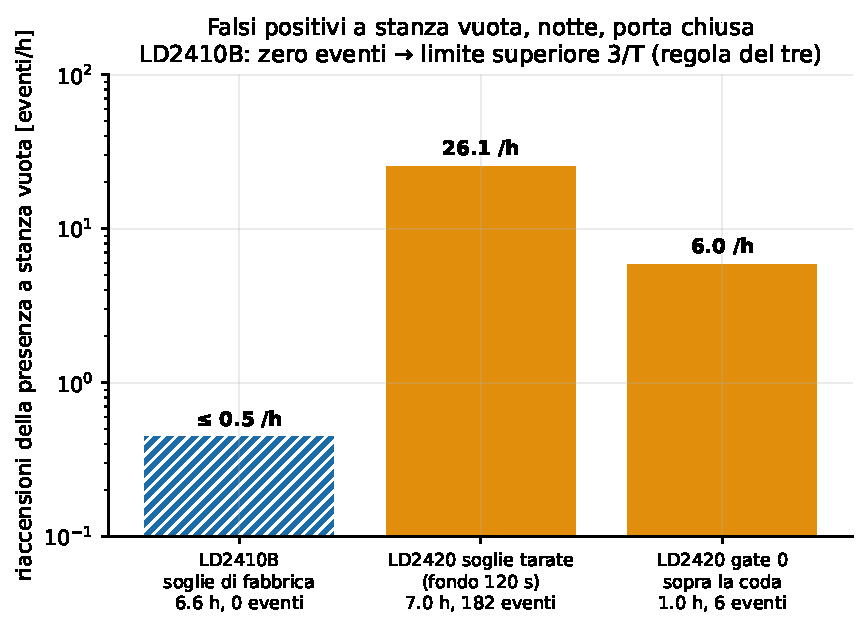
\includegraphics[width=\linewidth]{figures/fig18_falsi_positivi}
\caption{Falsi positivi a stanza vuota, di notte, in scala logaritmica. L'\ldb\ a
soglie di fabbrica non produce eventi in 6,6~h, quindi è riportato il limite superiore
$3/T$. L'\ldc\ con le soglie tarate sul fondo misurato produce 26 riaccensioni/h in
7~h di notte, che scendono a 6/h con il gate~0 portato sopra la coda del rumore,
misurati però in 1~h di giorno. I
conteggi della figura usano lo scarto di 60~s degli script e differiscono di poco da
quelli del testo, che usano la finestra del registro.}
\label{fig:falsi-positivi}

\end{figure}

\section{La persona ferma}
\label{sec:persona-ferma}

È lo scenario che risponde alla domanda di partenza. Il soggetto siede immobile a
2,30~m dai sensori, con la sola respirazione spontanea, per cinque trial da 302~s
utili a 27\,\textdegree C. I 7554 campioni con presenza reale danno il risultato della
Tabella~\ref{tab:fermo-seduto}.

\begin{table}[htbp]
\centering
\caption{Persona ferma seduta a 2,30~m, cinque trial da 302~s.}
\label{tab:fermo-seduto}

\small
\begin{tabular}{@{}lrr@{}}
\toprule
 & \textbf{PIR \pir} & \textbf{Radar \ldb} \\
\midrule
Falsi negativi & $99{,}78 \pm 0{,}49\,\%$ & $\mathbf{0{,}00 \pm 0{,}00\,\%}$ \\
Trial con falsi negativi al 100\,\% & 4 su 5 & 0 su 5 \\
Campioni con presenza rilevata & $\sim$17 su 7554 & 7554 su 7554 \\
\bottomrule
\end{tabular}
\end{table}

Con una persona viva a 2,3~m in campo libero, il PIR è rimasto muto per cinque minuti in quattro trial su cinque. Non è un esito inatteso, perché è ciò che il
principio del piroelettrico prevede (Sezione~\ref{subsec:pir-principio}), e ne viene quantificata la dispersione nello scenario di progetto. La
Figura~\ref{fig:timeline-sotto-banco} mostra l'andamento nel tempo di un trial in questa
geometria e di uno nella geometria del progetto DIPME (Sezione~\ref{sec:sotto-banco}).

\begin{figure}[htbp]
\centering
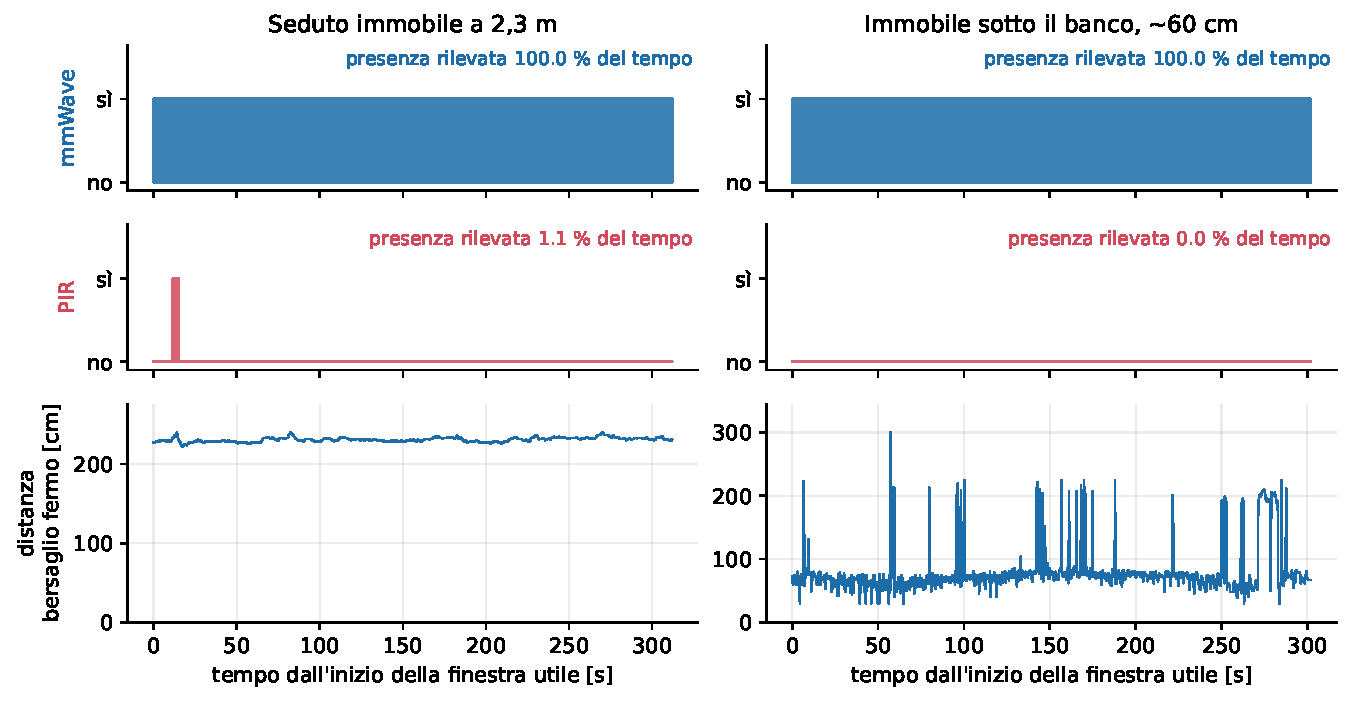
\includegraphics[width=\linewidth]{figures/fig02_timeline_sotto_banco}
\caption{Presenza dichiarata dai due sensori su una persona immobile, in due
geometrie. A sinistra il soggetto seduto a 2,3~m, a destra rannicchiato sotto il
banco a circa 60~cm, cinque minuti ciascuno. Il radar è continuo, il PIR produce al
più un impulso isolato. La terza riga è la distanza riportata dal radar sul bersaglio
fermo, stabile entro 1,5~cm da seduto e molto più rumorosa sotto il piano.}
\label{fig:timeline-sotto-banco}

\end{figure}

\subsection{Che cosa misura il bit del PIR}
\label{sec:interpretazione-pir}
\label{sec:jumper}

La percentuale di campioni in cui il PIR è alto va letta sapendo come nasce. In
posizione L l'uscita è un monostabile a durata fissa. Su tutte le sessioni acquisite
in quella configurazione sono stati contati 195 impulsi con durata media
$3{,}46 \pm 0{,}09$~s, tutti fra 3,4 e 3,6~s e nessuno oltre 5~s, anche nei trial
in cui il soggetto si muoveva per cinque minuti (Figura~\ref{fig:impulsi-pir}). La
percentuale è quindi il numero di eventi moltiplicato per la ritenuta, cioè un
conteggio di eventi travestito da frazione di tempo. In posizione H gli impulsi si
concatenano finché il movimento continua, fino a coprire un intero trial di 62~s, e la
percentuale diventa allora una vera frazione di tempo con movimento rilevato. Il
significato delle due modalità è descritto nella Sezione~\ref{subsec:pir-principio}.

\begin{figure}[htbp]
\centering
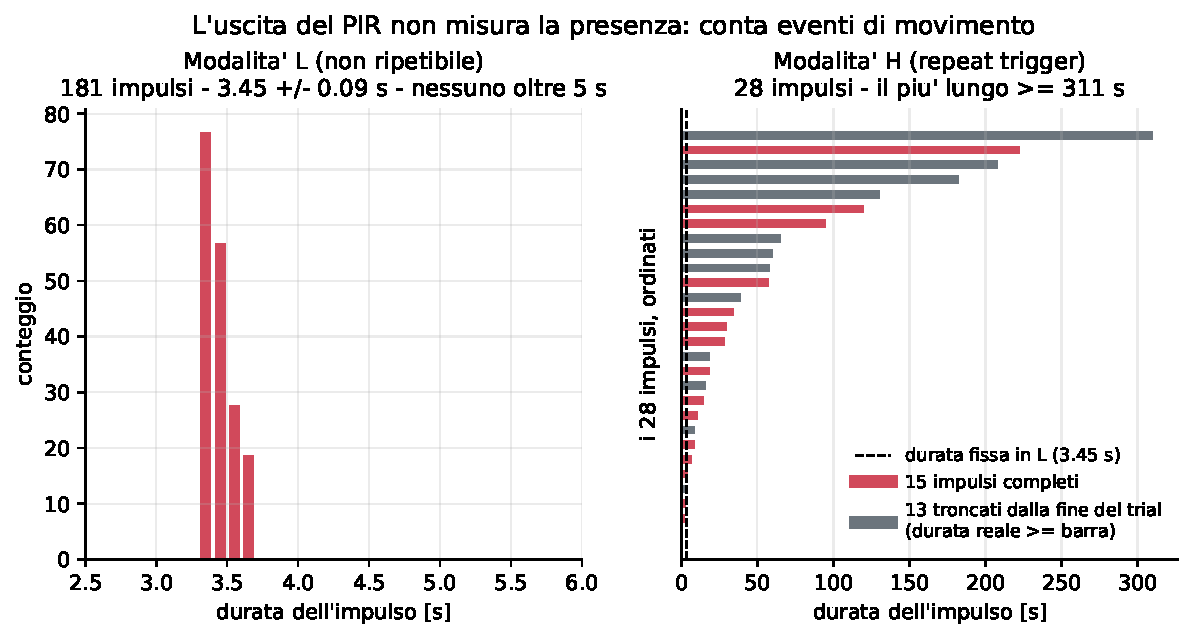
\includegraphics[width=\linewidth]{figures/fig07_impulsi_pir}
\caption{Struttura degli impulsi del PIR nelle due serie con movimento continuo, il cammino sul posto a 1~m e i movimenti sotto il banco, che in L contengono 181 dei 195 impulsi. In L la durata è fissa, in H il ritrigger concatena gli impulsi.}
\label{fig:impulsi-pir}

\end{figure}

Come anticipato nella Sezione~\ref{sec:c3-3-3}, la prima parte della campagna è stata acquisita in posizione L, e le serie del cammino sul posto a 1~m e dei micro-movimenti sotto il banco sono state ripetute in H e sono quelle riportate in questo capitolo. Anche se le altre serie non richiedevano una ripetizione, perché il ponticello agisce solo dopo un trigger e uno scenario in cui il PIR non ha prodotto eventi non può cambiare, sono stati comunque ripetuti in H, per verifica, il cammino a 2~m (0,00\,\% in entrambe le posizioni) e l'immobilità sotto il banco (0,10\,\% in L, 1,32\,\% in H).

\section{Il rilevamento al variare del movimento}
\label{sec:dose-risposta}
\label{sec:pir-movimento}

Le due prove di questa sezione variano una sola grandezza alla volta. La prima varia la quantità di movimento a distanza fissa, con una curva dose-risposta a 1~m, la seconda il tipo di movimento a parità di distanza, confrontando il cammino sul posto con l'attraversamento.

\subsection{Quantità di movimento}
\label{sec:dose-risposta-1m}

Il soggetto è in piedi a 1~m, la distanza più favorevole al PIR fra quelle provate, così che il confronto non sia costruito a suo sfavore. Il ponticello è in H, il montaggio è lo stesso in tutte le condizioni e la quantità di movimento assume tre livelli, con cinque trial ciascuno (Tabella~\ref{tab:dose-risposta} e Figura~\ref{fig:dose-risposta}).

\begin{table}[htbp]
\centering
\caption{Curva dose-risposta a 1~m, ponticello in H, cinque trial per condizione. Le due colonne
di destra sono grandezze del radar, riprese nel Capitolo~\ref{chap:vitalita}.}
\label{tab:dose-risposta}

\small
\begin{tabular}{@{}lrrrrr@{}}
\toprule
\textbf{Condizione} & \textbf{PIR} & \textbf{dev.\ rel.} & \textbf{Radar} &
\textbf{Energia mov.} & \textbf{Disp.\ dist.} \\
\midrule
Immobile          & $1{,}52 \pm 1{,}03\,\%$   & $68\,\%$ & $\mathbf{100\,\%}$ & 68,6 & 21,3~cm \\
Micro-movimenti   & $51{,}60 \pm 21{,}72\,\%$ & $\mathbf{42\,\%}$ & $\mathbf{100\,\%}$ & 84,4 & 16,4~cm \\
Cammino sul posto & $85{,}20 \pm 11{,}52\,\%$ & $14\,\%$ & $\mathbf{100\,\%}$ & 99,3 & 10,4~cm \\
\bottomrule
\end{tabular}
\end{table}

\begin{figure}[htbp]
\centering
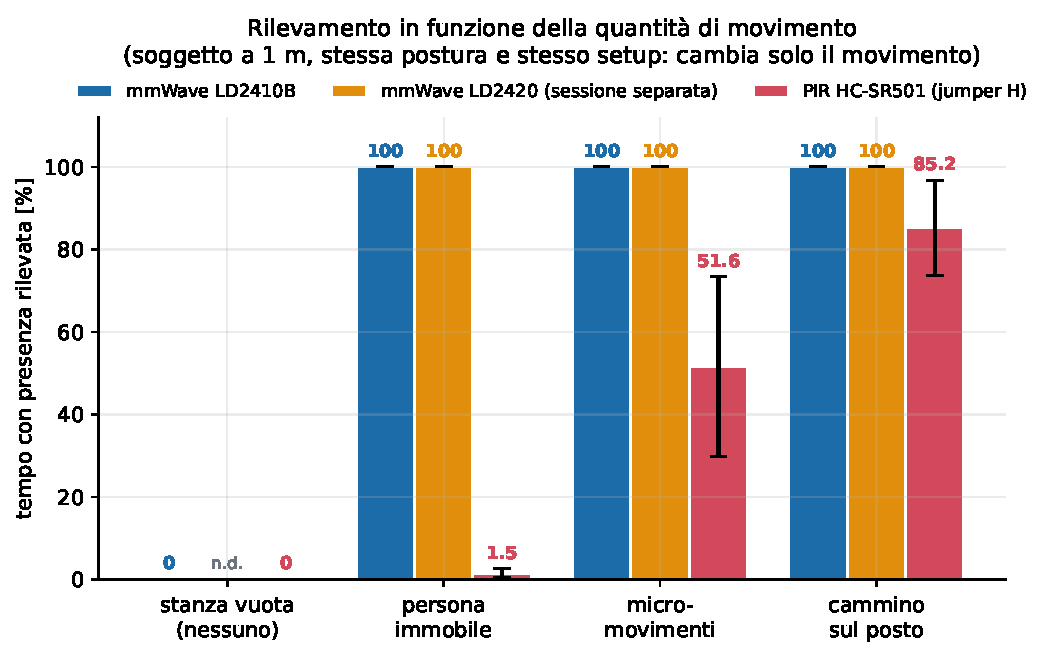
\includegraphics[width=\linewidth]{figures/fig01_dose_risposta}
\caption{La curva dose-risposta a 1~m. Il PIR passa dall'1,5 all'85\,\%,
con la dispersione massima nella zona intermedia. Il radar resta al 100\,\% in tutte e tre le condizioni.}
\label{fig:dose-risposta}

\end{figure}

Il fallimento del PIR sulla persona ferma dipende quindi dall'immobilità del soggetto e non dalla distanza, dalla configurazione o dalla taratura, che fra le righe restano invariate. Da immobile il PIR produce due soli impulsi in 1010~s di acquisizione.

Per un'applicazione di soccorso il dato più rilevante è la dispersione della condizione intermedia, $\pm 21{,}72$ punti su una media di 51,60, perché due trial identici per l'operatore danno risultati molto diversi. Vicino alla propria soglia il PIR diventa imprevedibile e non permette di interpretare correttamente l'assenza di segnale.

Le ultime due colonne della
Tabella~\ref{tab:dose-risposta} sono un risultato a sé. L'energia del bersaglio in movimento
cresce con la quantità di movimento, mentre la dispersione della distanza cala, perché un'eco più forte dà una stima più stabile.
Sono due grandezze continue e monotone misurate a geometria costante, e su di esse
poggia l'indice di vitalità del Capitolo~\ref{chap:vitalita}.

\subsection{Tipo di movimento}
\label{sec:attraversamento}

Il cammino sul posto è stato ripetuto
a 1, 2, 3, 4 e 5~m, con cinque trial per distanza. A 1~m il PIR rileva l'85,2\,\% del
tempo, mentre da 2~m in poi resta a zero. Sono venti
trial consecutivi al 100\,\% di falsi negativi con un soggetto in movimento continuo
davanti al sensore, e il crollo fra 1 e 2~m non è graduale. Questo esito è in aperto
contrasto con la portata di 3--7~m dichiarata dal costruttore, ma da solo non
distingue fra due spiegazioni, cioè il tipo di movimento oppure un esemplare guasto o
tarato male. Per decidere, il soggetto ha ripetuto la prova camminando in modo
continuo trasversalmente all'asse del sensore, a distanza costante. Tutto il resto è
rimasto invariato (ponticello in H e trimmer di sensibilità nella stessa posizione),
con tre trial per distanza. Il risultato è in Figura~\ref{fig:tipo-movimento}.

\begin{figure}[htbp]
\centering
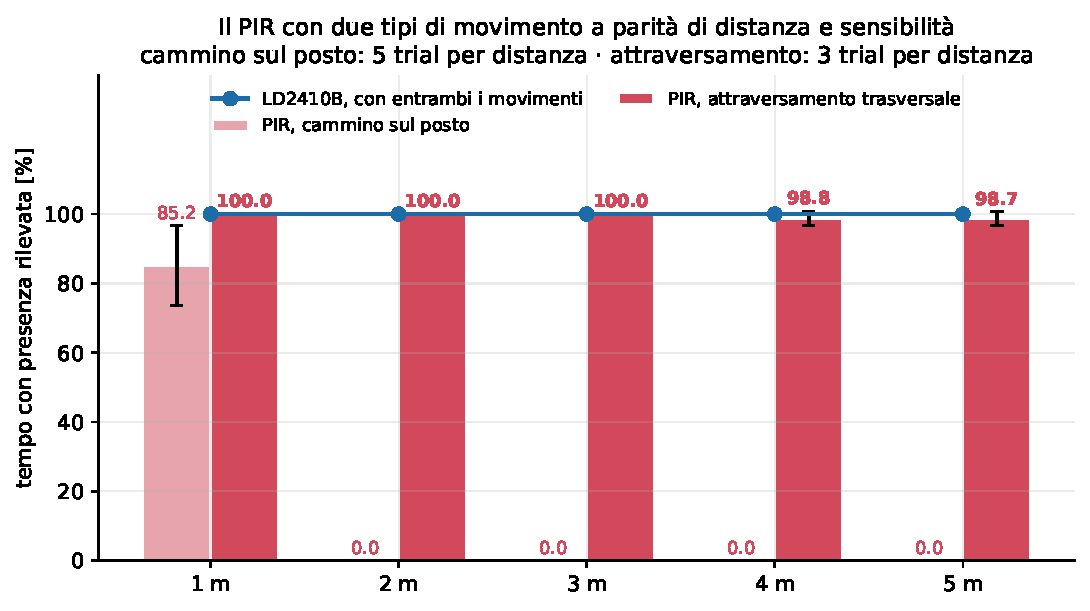
\includegraphics[width=\linewidth]{figures/fig28_tipo_movimento}
\caption{Il PIR con due tipi di movimento. A parità di distanza e sensibilità, il cammino sul posto è rilevato solo a 1~m (85\,\%) e mai da 2~m in su.
L'attraversamento trasversale è rilevato al 99--100\,\% da 1 a 5~m. Il radar è al
100\,\% con entrambi i movimenti. Il ponticello è in H, tranne che nelle serie sul posto a 3--5~m, acquisite in posizione L, dove il PIR non produce eventi e il ponticello non cambia nulla (Sezione~\ref{sec:interpretazione-pir}).}
\label{fig:tipo-movimento}

\end{figure}

Un sensore che rileva un attraversamento a 5~m nel 98,7\,\% dei campioni non è né
guasto né poco sensibile, e la portata dichiarata risulta confermata. A decidere è quindi il tipo di movimento, come prevede la geometria della lente di Fresnel (Sezione~\ref{subsec:fresnel}). Lo conferma una prova a 1~m con quattro movimenti diversi, per i quali l'energia in movimento del radar è rimasta fra 96,5 e 98,1, cioè la stessa quantità di movimento. Il PIR è passato dal 2\,\% con il movimento delle braccia al 100\,\% con l'oscillazione laterale del busto da seduto, che è una traversata in miniatura. I due sensori misurano quindi grandezze diverse, il radar la quantità di movimento e il PIR il passaggio da una zona all'altra della lente.

Per il progetto la conseguenza è diretta. Il movimento per cui il PIR è progettato,
attraversare un varco o percorrere un corridoio, è l'opposto di quello di una persona
intrappolata sotto un arredo, che, se si muove, lo fa sul posto. Il limite è quindi strutturale rispetto allo scenario.

\section{Lo scenario DIPME: la persona sotto il banco}
\label{sec:sotto-banco}
\label{sec:gate-sotto-banco}

È lo scenario che replica la condizione del progetto. I sensori sono fissati sotto il
piano di un tavolo e il soggetto è rannicchiato sotto di esso a 50--60~cm
(Figura~\ref{fig:geometrie}b). Sono stati acquisiti cinque trial da 302~s utili in due
condizioni, immobilità e presenza di micro-movimenti, entrambe con il ponticello del
PIR in H (Figura~\ref{fig:dipme-tre-sensori}).

\begin{figure}[htbp]
\centering
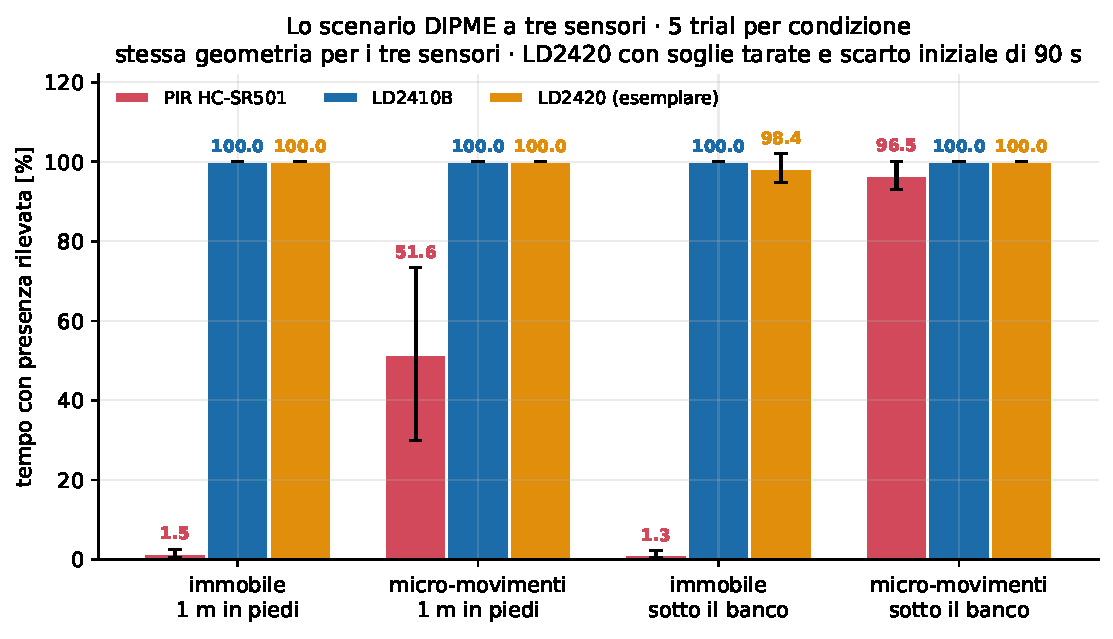
\includegraphics[width=\linewidth]{figures/fig19_dipme_tre_sensori}
\caption{Lo scenario DIPME a tre sensori, cinque trial per condizione. L'\ldc\ è stato provato nella stessa geometria, con soglie tarate e scarto di 90~s. I due radar sono al 100\,\% in tutte le condizioni, salvo l'\ldc\ al 98,4\,\%
da immobile sotto il banco per un rilascio di 24~s in un trial su cinque. Il PIR
passa dall'1--2\,\% da fermo al 52--97\,\% con i micro-movimenti.}
\label{fig:dipme-tre-sensori}

\end{figure}

Sotto il banco il contrasto è ancora più netto che a 1~m. Con i micro-movimenti il PIR
rileva il $96{,}52 \pm 3{,}60\,\%$ del tempo, da immobile l'$1{,}32 \pm 0{,}86\,\%$.
A 60~cm il PIR è un rilevatore di movimento quasi perfetto e resta cieco alla persona
ferma. L'\ldb\ è al 100\,\% in entrambe le condizioni su 7554 campioni per
condizione. L'\ldc\ è al 100\,\% con i micro-movimenti e al $98{,}4 \pm 3{,}6\,\%$
da immobile, con un solo rilascio di 24~s in un trial.

\paragraph{Il radar rileva bene ma localizza male.} La dispersione della distanza
entro il trial vale 14--24~cm sotto il banco, contro $1{,}48 \pm 0{,}77$~cm sul
soggetto seduto a 2,3~m (Figura~\ref{fig:timeline-sotto-banco}), cioè circa dieci volte
peggio su un bersaglio immobile più vicino. Per il progetto è irrilevante, perché al
soccorritore serve sapere se c'è qualcuno sotto quel banco e non a quanti centimetri,
ma esclude l'uso della distanza come misura fine in questa geometria. Gli sbalzi
verso 200--300~cm visibili in Figura~\ref{fig:timeline-sotto-banco} riguardano dallo 0,3 al
7,4\,\% dei campioni nei cinque trial e avvengono con il canale in movimento meno
attivo del solito e con il PIR a zero. Non sono movimenti del soggetto, perché i file terminano prima che l'operatore si alzi e i primi 40~s sono scartati, ma il canale stazionario che si aggancia a un riflesso lontano. La lettura per gate spiega perché la localizzazione è rumorosa. Sull'\ldb\ i gate stazionari 0 e 1
sono strutturalmente nulli (Sezione~\ref{sec:c3-5-2}) e la presenza è retta dai gate 2
e 3, con un'energia che resta a 24 anche al gate~8 contro 6,5 nello scenario da
seduto. Sull'\ldc\ la presenza da immobile è retta dal gate~2 (70--140~cm) e non dal
gate~1 in cui la persona sta. Lo stesso fenomeno compare su due moduli diversi,
verosimilmente per cammini multipli sotto il piano. È una spiegazione coerente, non
una misura, perché il segnale grezzo non è accessibile. Resta comunque acquisito il
punto operativo, cioè che sotto il metro l'indice di vitalità deve usare i canali in
movimento (Capitolo~\ref{chap:vitalita}).

\section{Accuratezza della distanza ed energia}
\label{sec:distanza}

\subsection{Accuratezza della distanza}
\label{sec:distanza-accuratezza}

I 25 trial di cammino sul posto a 1--5~m caratterizzano la misura di distanza dell'\ldb\ (Tabella~\ref{tab:distanza}, Figura~\ref{fig:distanza-regressione}).

\begin{table}[htbp]
\centering
\caption{Accuratezza della distanza riportata dall'\ldb, 25 trial (5 distanze $\times$
5 ripetizioni, 62~s utili ciascuno). ``Misurata'' è la media fra trial con la sua
deviazione standard, ``residuo'' lo scarto dalla retta dell'Equazione~\ref{eq:regressione},
``disp.\ entro trial'' la deviazione standard della distanza dentro un trial, mediata
sui cinque. L'energia è il valore medio del bersaglio in movimento.}
\label{tab:distanza}

\small
\begin{tabular}{@{}rrrrrrr@{}}
\toprule
\textbf{Reale} & \textbf{Misurata} & \textbf{Errore} & \textbf{Err.\ rel.} &
\textbf{Residuo} & \textbf{Disp.\ entro trial} & \textbf{Energia} \\
\midrule
1~m & $99{,}48 \pm 2{,}61$~cm  & $-0{,}52$~cm & $-0{,}5\,\%$ & $-3{,}0$~cm & $10{,}4$~cm & 99,0 \\
2~m & $211{,}22 \pm 0{,}77$~cm & $+11{,}22$~cm & $+5{,}6\,\%$ & $+4{,}9$~cm & $14{,}3$~cm & 85,1 \\
3~m & $309{,}76 \pm 1{,}13$~cm & $+9{,}76$~cm & $+3{,}3\,\%$ & $-0{,}4$~cm & $17{,}5$~cm & 54,4 \\
4~m & $411{,}84 \pm 2{,}76$~cm & $+11{,}84$~cm & $+3{,}0\,\%$ & $-2{,}1$~cm & $26{,}4$~cm & 35,1 \\
5~m & $518{,}20 \pm 2{,}13$~cm & $+18{,}20$~cm & $+3{,}6\,\%$ & $+0{,}5$~cm & $11{,}7$~cm & 27,6 \\
\bottomrule
\end{tabular}
\end{table}

\begin{figure}[htbp]
\centering
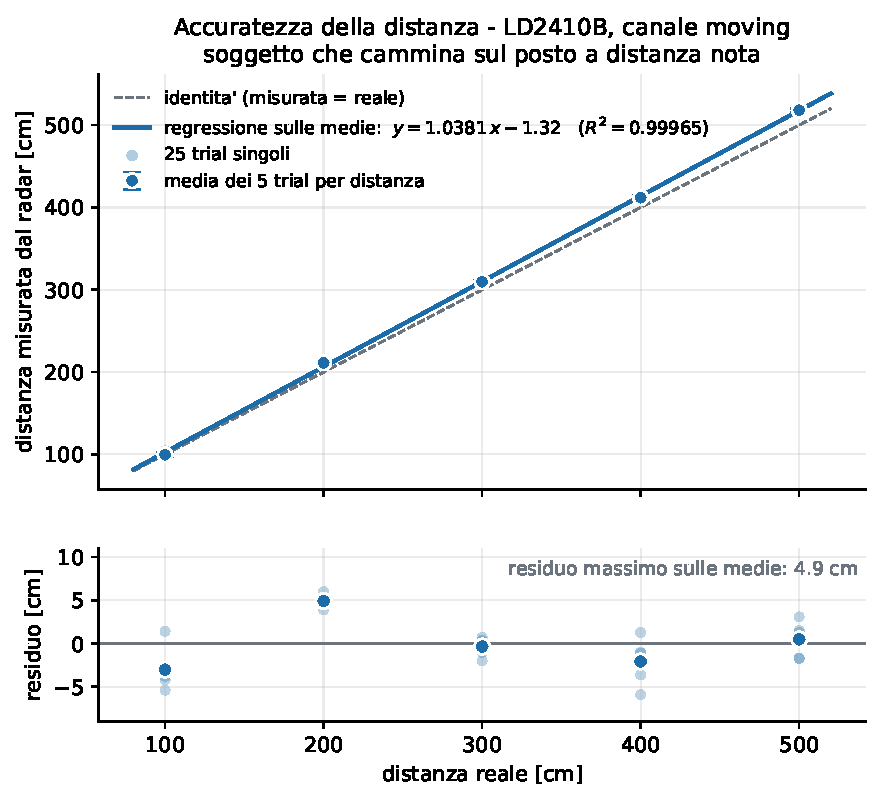
\includegraphics[width=\linewidth]{figures/fig04_distanza_regressione}
\caption{Accuratezza della distanza dell'\ldb, 25 trial fra 1 e 5~m. La retta è calcolata sulle cinque medie per distanza, sui 25 trial singoli $R^2$ sarebbe 0,99949 anziché 0,99965.}
\label{fig:distanza-regressione}

\end{figure}

La regressione lineare fra distanza misurata e reale dà
\begin{equation}
d_{\text{misurata}} = 1{,}0381 \cdot d_{\text{reale}} - 1{,}32~\text{cm},
\qquad R^2 = 0{,}99965.
\label{eq:regressione}
\end{equation}
Il radar è estremamente lineare, con residui dalla retta non superiori a 4,9~cm su
tutto il range. L'errore è quasi interamente di scala ($+3{,}81\,\%$) con offset
trascurabile, e questo spiega perché l'errore grezzo cresce con la distanza, da
$-0{,}5$~cm a 1~m a $+18{,}2$~cm a 5~m. È correggibile dividendo la lettura per 1,0381. I dati non
permettono di attribuire il $+3{,}81\,\%$ al modulo piuttosto che al riferimento con
cui sono state segnate le distanze sul pavimento, e per farlo servirebbe un
distanziometro indipendente.

La dispersione entro il trial (10--26~cm) non è rumore del sensore, ma l'oscillazione
reale del busto di chi cammina sul posto, come mostra il confronto con l'1,48~cm del
soggetto seduto immobile. In quello scenario la variabilità fra trial della distanza
media ($\pm 2{,}38$~cm) è maggiore di quella entro il trial, quindi il fattore
limitante è come il soggetto si siede e non lo strumento.

\subsection{Energia del bersaglio}
\label{sec:energia-distanza}

\begin{figure}[htbp]
\centering
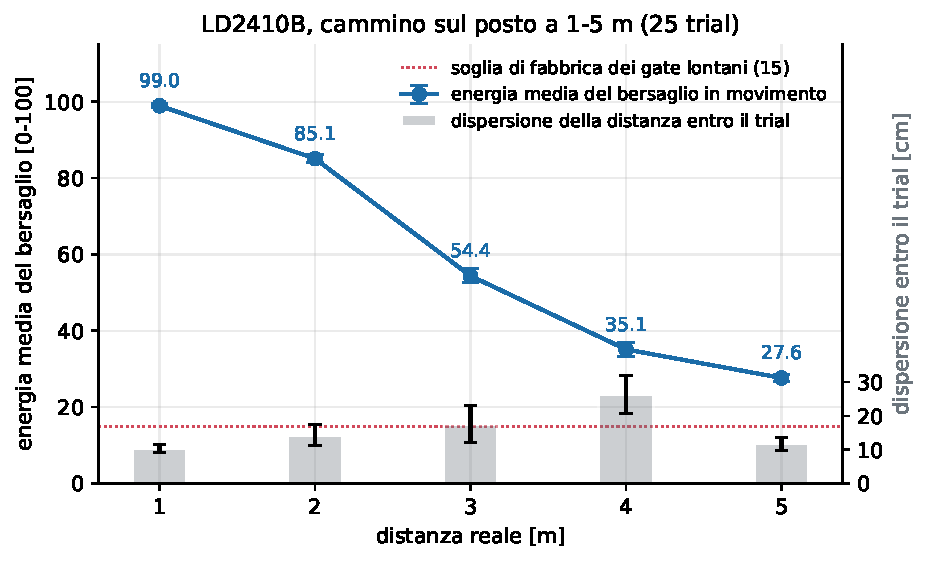
\includegraphics[width=\linewidth]{figures/fig05_energia_distanza}
\caption{Energia del bersaglio in movimento e dispersione della distanza entro il
trial in funzione della distanza, 25 trial. A 5~m l'energia (27,6) è ancora quasi il
doppio della soglia di fabbrica dei gate lontani.}
\label{fig:energia-portata}

\end{figure}

L'energia media del bersaglio decade da 99 a 1~m a 28 a 5~m
(Figura~\ref{fig:energia-portata}). Il decadimento è molto più lento della dipendenza
$1/D^4$ della potenza ricevuta da un bersaglio puntiforme, perché il valore non è una potenza ma un indice normalizzato prodotto da un'elaborazione interna non documentata (Sezione~\ref{sec:c3-5-1}). Per questo se ne usa
la monotonia e non il valore assoluto in termini fisici. Il range di 1--5~m è un limite
della stanza e non del sensore, e la portata oltre i 5~m è misurata in corridoio in
Sezione~\ref{sec:portata-massima}.

\subsection{Il secondo radar e il PIR}
\label{sec:distanza-ld2420}

Il PIR non compare in questa sezione perché
non misura né una distanza né un'energia, e il suo dato è un bit. L'\ldc\ riporta una
distanza solo sul bersaglio in movimento e, sull'esemplare in dotazione, solo da
vicino. In venti trial di cammino sul posto da 0,5 a 2~m la distanza riportata vale
$59 \pm 5$~cm a 0,5~m e $121 \pm 9$~cm a 1~m, con errori di $+9$ e $+21$~cm e da 4 a
38 valori distinti al minuto. A 1,5 e 2~m il modulo riporta un solo valore stantio per
trial, quindi una retta di calibrazione non è costruibile. Sulla persona immobile
riporta il valore di riposo (2--5~cm) con la presenza al 100\,\%, come dichiara il
produttore. Anche l'energia del gate della persona non è una grandezza graduata su
questo esemplare, come mostra la dose-risposta ripetuta in Sezione~\ref{sec:ld2420-risultati}.

\section{Latenze di rilevamento e di rilascio}
\label{sec:latenza}
\label{sec:rilascio}

L'acquisizione parte con la stanza vuota oppure con il soggetto presente, che
rispettivamente entra o esce a $t = 30$~s, istante annunciato dallo script di
acquisizione (Sezione~\ref{sec:protocollo-groundtruth}). Sono stati acquisiti dieci
trial all'ingresso e cinque all'uscita, tutti validi, con nessun sensore attivo prima
dell'evento. I risultati sono in Tabella~\ref{tab:latenze} e Figura~\ref{fig:latenze}.

\begin{table}[htbp]
\centering
\caption{Latenze all'ingresso e tempo di rilascio all'uscita. \ldb\ e PIR letti
nello stesso trial (10 all'ingresso, 5 all'uscita), con la differenza appaiata
calcolata trial per trial e nessuna riaccensione dopo il rilascio. L'\ldc\ è misurato
in una sessione separata (5 trial all'ingresso, 3 all'uscita) con il ritardo di
scomparsa portato da 30 a 5~s come sull'\ldb. Il PIR non era cablato, quindi manca la
differenza appaiata.}
\label{tab:latenze}

\small
\begin{tabularx}{\linewidth}{@{}lrrrX@{}}
\toprule
\textbf{Grandezza} & \textbf{\ldb} & \textbf{PIR \pir} & \textbf{\ldc} & \textbf{Nota} \\
\midrule
Latenza all'ingresso & $5{,}36 \pm 0{,}30$~s & $5{,}96 \pm 0{,}31$~s & $7{,}28 \pm 1{,}40$~s &
  latenza operativa, non del solo sensore \\
Differenza appaiata \ldb\ $-$ PIR & \multicolumn{2}{c}{$\mathbf{-0{,}60 \pm 0{,}35}$~\textbf{s}} & --- &
  il radar rileva per primo in 10 trial su 10 \\
Tempo di rilascio all'uscita & $\mathbf{18{,}36 \pm 0{,}54}$~s & $12{,}96 \pm 1{,}40$~s & $7{,}7 \pm 0{,}5$~s &
  \ldb\ più lento del PIR di $5{,}40 \pm 0{,}67$~s. \ldc\ con ritardo 5~s \\
\bottomrule
\end{tabularx}
\end{table}

\begin{figure}[htbp]
\centering
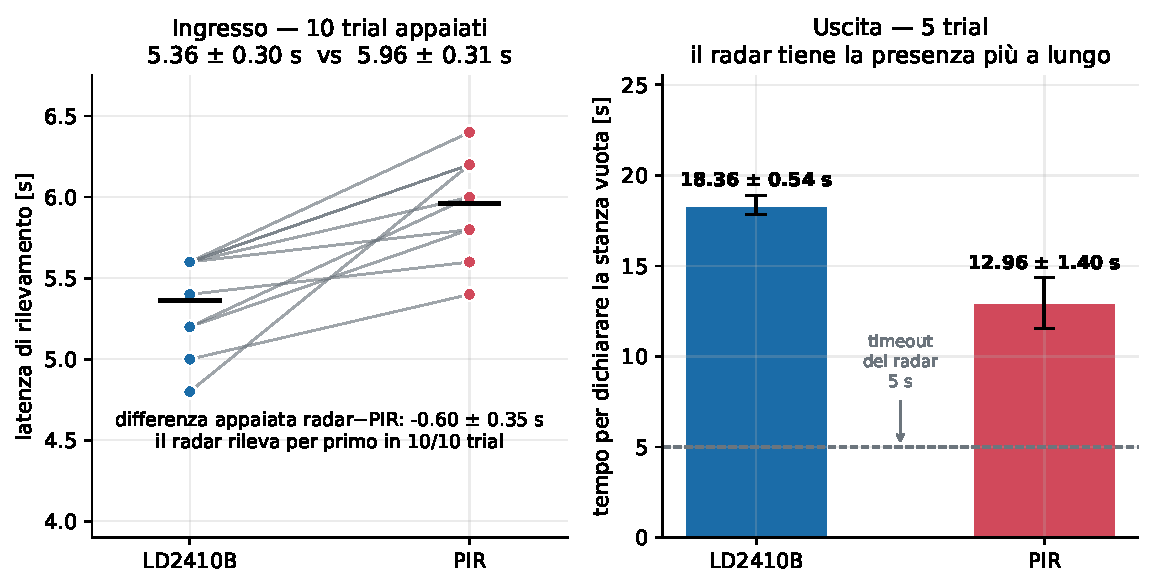
\includegraphics[width=\linewidth]{figures/fig06_latenze}
\caption{A sinistra le latenze appaiate all'ingresso. A destra la latenza di rilascio all'uscita, dove il radar impiega 18~s
a dichiarare la stanza vuota contro un timeout configurato di 5.}
\label{fig:latenze}

\end{figure}

\paragraph{Ingresso.} Le latenze assolute intorno a 5--6~s sono una latenza operativa, che comprende il tragitto e il tempo di reazione del soggetto, e la grandezza pulita è la differenza appaiata (Sezione~\ref{sec:metriche-elenco}). Il valore $-0{,}60 \pm 0{,}35$~s è una proprietà dei
sensori, con errore standard della media di 0,11~s. Il segno è concorde in tutti e
dieci i trial, con probabilità $\approx 0{,}002$ sotto l'ipotesi di equivalenza. Con
il campionamento a 5~Hz le singole differenze valgono da uno a sette campioni, quindi
la conclusione poggia sulla concordanza del segno e non sull'ampiezza di una misura. Ci si
attendeva il contrario, perché attraversare una porta è lo stimolo trasversale per
cui la lente di Fresnel è progettata. Una spiegazione plausibile, non dimostrata, è
che il radar agganci il soggetto ancora in avvicinamento grazie ai 6~m di portata.

\paragraph{Uscita.} Qui il radar è nettamente più lento, $5{,}40 \pm 0{,}67$~s in
più del PIR, un effetto otto volte la propria incertezza già con cinque trial. Il
tempo di rilascio include il tempo di uscita dal campo, e il PIR può servire da
cronometro, perché la sua uscita ricade $3{,}46$~s dopo l'ultimo trigger. Il soggetto esce
quindi dal campo circa 9,5~s dopo l'annuncio, e la coda propria del radar vale circa
$18{,}36 - 9{,}5 \approx 8{,}9$~s. È una stima, perché i campi dei due sensori non
coincidono, ma concorda con altre due osservazioni indipendenti (10 e 12~s). Il
timeout di presenza letto dal modulo vale invece 5~s (Tabella~\ref{tab:c3-6}), quindi
il parametro configurato non descrive il comportamento osservato. Per il progetto
significa che una stanza appena liberata risulta occupata per quasi dieci secondi.

\paragraph{Il secondo radar.} Sullo stesso percorso l'\ldc\ rileva l'ingresso in
$7{,}28 \pm 1{,}40$~s su cinque trial, quasi due secondi dopo l'\ldb\ e con una
dispersione quattro volte maggiore. La ragione è che aggancia il soggetto solo entro
circa 1~m, mentre l'\ldb\ lo aggancia in avvicinamento a 4--5~m. Il rilascio va
letto insieme al suo parametro. Con il ritardo di scomparsa di fabbrica, 30~s, il
modulo restava in presenza per 87--120~s dopo l'uscita, perché basta un superamento
della soglia di mantenimento ogni mezzo minuto a riarmare il ritardo
(Sezione~\ref{sec:ld2420-risultati}). Portato a 5~s come sull'\ldb, il rilascio scende a $7{,}7 \pm 0{,}5$~s. La prova ha chiarito anche l'unità del parametro, su cui manuale e documento di protocollo si contraddicono, e ha mostrato che sono secondi. Il confronto a parametro pari (7,7 contro 18,4~s) è però dominato
dal tempo di uscita dal campo (1--2~m di portata contro 5--6), quindi non significa
che l'\ldc\ rilasci più in fretta.

\section{Copertura angolare e selettività fra banchi}
\label{sec:angolare}

Nell'architettura del progetto ogni arredo ha il proprio sensore, che deve riportare
il proprio occupante e non quello del banco accanto. Lo strumento offerto dall'\ldb\ è
il gate massimo, che con la regola documentata di 75~cm per gate porta la portata a
150~cm quando vale 2 (Tabella~\ref{tab:c3-6}). Il gate limita però la distanza e non
l'angolo, quindi la domanda è doppia. Bisogna capire se il limite di distanza funziona
e se il vicino laterale viene visto.

\subsection{Selettività con gate massimo 2}
\label{sec:selettivita}

Sono stati provati quattro scenari con
soggetti sempre fermi, con tre trial da 182~s ciascuno (Figura~\ref{fig:selettivita}).
L'occupante a 1~m sull'asse è rilevato al 100\,\%, mentre una persona a 3~m sull'asse,
oltre il taglio, è rilevata allo 0,00\,\%. Anche una persona a 1~m a 90\textdegree\ è rilevata allo 0,00\,\% a regime, e il $24{,}8 \pm 19{,}6\,\%$ che si ottiene con lo scarto ordinario di 20~s è la coda del posizionamento della Figura~\ref{fig:transitorio}. Con l'occupante e il vicino insieme, nessuna grandezza dell'occupante cambia
oltre $2\,\sigma$ (la distanza di 4~cm, l'energia di 4 punti).

\begin{figure}[htbp]
\centering
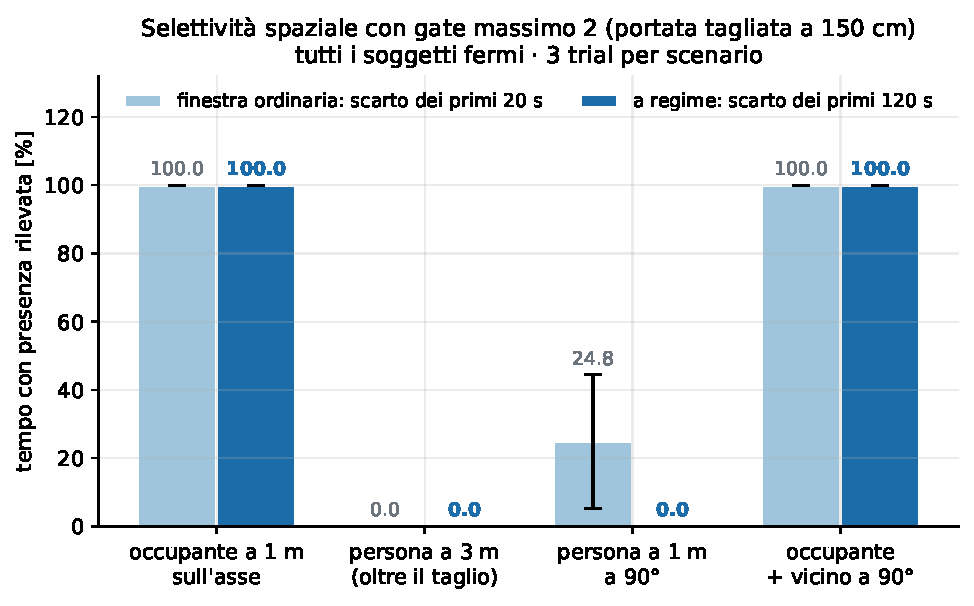
\includegraphics[width=\linewidth]{figures/fig09_selettivita}
\caption{Selettività spaziale con gate massimo 2 (150~cm), tre trial per scenario.
Le barre chiare usano lo scarto ordinario dei primi 20~s, quelle scure lo scarto di
120~s (a regime). A 3~m zero rilevamenti. Il vicino a 90\textdegree\ fermo non è
rilevato a regime, e il 24,8\,\% della finestra ordinaria è la coda del
posizionamento (Figura~\ref{fig:transitorio}).}
\label{fig:selettivita}

\end{figure}

\subsection{Copertura angolare}
\label{sec:angolare-copertura}

Il soggetto siede su un arco di raggio 1~m a sei
azimut (0, 45, 60, 75, 90 e 120\textdegree), con la sedia rivolta verso i sensori a
ogni posizione, e oscilla lateralmente il busto con ampiezza costante. Il gate massimo
vale 2 e i trial sono da uno a tre per angolo (Figura~\ref{fig:angolare-due-radar}). L'\ldb\ rileva al
100\,\% fino a 90\textdegree\ compresi, con l'energia che cala di due punti soli fra
l'asse e i 90\textdegree\ (da 96,5 a 94,3), e crolla fra 90 e 120\textdegree. La
copertura eccede quindi nettamente i $\pm 60$\textdegree\ del manuale. Il PIR collassa prima,
dal 100\,\% sull'asse al 12\,\% a 90\textdegree\ e a zero a 120\textdegree. Fra 45 e
75\textdegree\ la dispersione fra trial è però dell'ordine dell'effetto, e a
45\textdegree\ i tre trial danno 100, 100 e 33\,\%, per cui le sole affermazioni
sostenibili riguardano i tre estremi. L'irripetibilità è essa stessa un risultato, lo stesso
comportamento già visto nella zona intermedia della dose-risposta. L'\ldc\ a 1~m ha il fascio utile fino a
circa 75\textdegree\ ed è al fondo a 90\textdegree, più stretto dell'\ldb\ e più largo
dei $\pm 45$ o $\pm 60$\textdegree\ del suo manuale. Il confine è coerente anche con
il margine ridotto del trasmettitore dell'esemplare (Sezione~\ref{sec:c3-2-6}).

\begin{figure}[htbp]
\centering
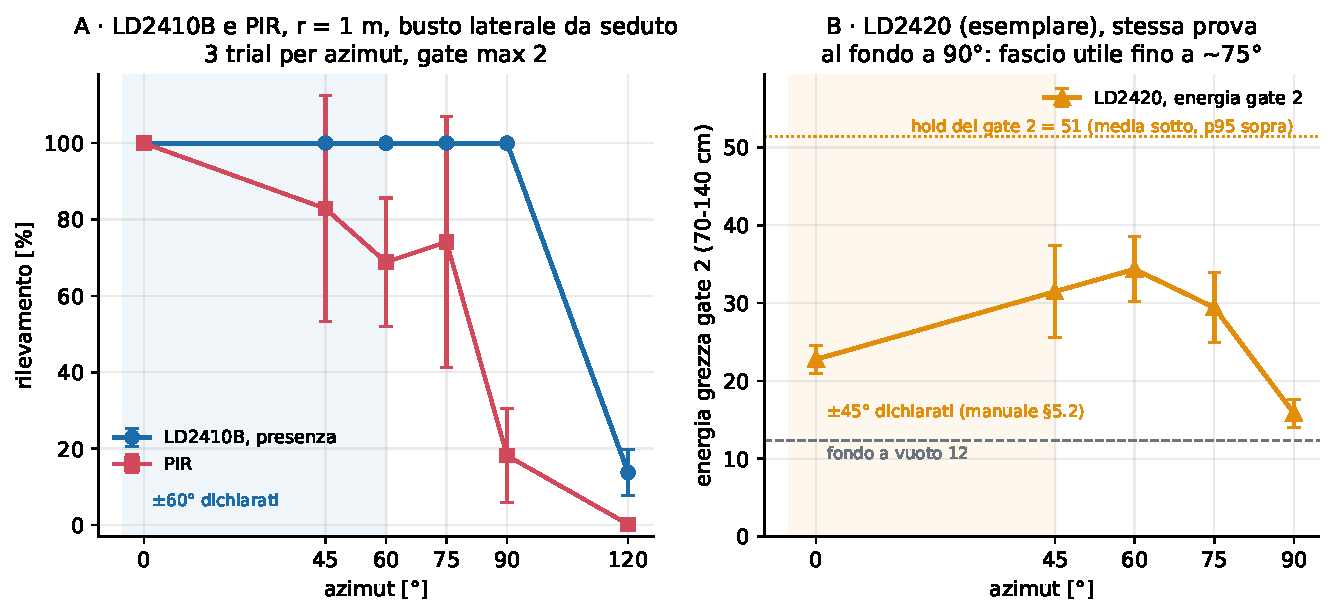
\includegraphics[width=\linewidth]{figures/fig20_angolare}
\vspace{3.0cm}% spazio per la didascalia nel margine (tufte non lo riserva)
\caption{Copertura angolare a 1~m, busto laterale da seduto. A: l'\ldb\ rileva al
100\,\% fino a 90\textdegree\ e crolla a 120, ben oltre i $\pm 60$\textdegree\
dichiarati. Il PIR non è ripetibile fra 45 e 75\textdegree. B: l'esemplare di \ldc\
è al fondo a 90\textdegree, fascio utile fino a circa 75.}
\label{fig:angolare-due-radar}

\end{figure}

\subsection{Selettività per configurazione}
\label{sec:selettivita-configurazione}

Incrociando le due
prove alla stessa distanza, allo stesso angolo e con lo stesso gate, il vicino a 1~m a
90\textdegree\ è rilevato allo 0\,\% se è fermo e al 100\,\% se si muove. Ciò che
nella prima prova sembrava selettività era la debolezza dell'eco di un corpo immobile. Il diagramma
di irradiazione non attenua abbastanza a 90\textdegree\ da escludere un bersaglio in
movimento, quindi un banco vuoto accanto a una persona che si muove risulta occupato.
La separazione fra arredi adiacenti va cercata nel montaggio fisico (orientamento verso
il basso, schermatura del lobo laterale) e non nei parametri del modulo. Fuori asse
l'\ldb\ sottostima anche la distanza (108, 107, 95, 94 e 85~cm da 0 a 90\textdegree\
sull'arco a 100~cm), verosimilmente perché aggancia la porzione di corpo più vicina.

\section{Due persone davanti al radar}
\label{sec:due-persone}

L'\ldb\ non ha risoluzione angolare, ma espone due canali indipendenti, uno per il
bersaglio in movimento e uno per quello stazionario, ciascuno con la propria distanza
(Sezione~\ref{sec:c3-1-4}). Nella prova la persona A è ferma a 2~m e la persona B a
4~m, sfalsate lateralmente di 50~cm per evitare l'ombra reciproca, con tre trial da
102~s per geometria. La variante in fila è acquisita come confronto. Un trial di controllo con B da sola
ferma a 4~m dà rilevamento al 100\,\% e distanza $388{,}9 \pm 3{,}7$~cm, quindi il
confondente della distanza è escluso (Tabella~\ref{tab:due-persone}, Figura~\ref{fig:due-persone}).

\begin{table}[htbp]
\centering
\caption{Capacità di separare due persone, su tre geometrie. ``B riportata'' è la
frazione di campioni in cui la persona lontana compare su almeno uno dei due canali,
riconosciuta dalla banda di distanza. Tre trial per geometria, 1833 campioni utili
ciascuna.}
\label{tab:due-persone}

\small
\begin{tabular}{@{}lrrrrr@{}}
\toprule
\textbf{Geometria} & \textbf{Entrambi i} & \textbf{B} & \textbf{Dist.} &
\textbf{Dist.} & \textbf{Presenza} \\
 & \textbf{canali attivi} & \textbf{riportata} & \textbf{staz.} & \textbf{mov.} &
\textbf{radar} \\
\midrule
B cammina, sfalsate di lato & $79{,}2\,\%$ & $\mathbf{73{,}8\,\%}$ & 212~cm & 389~cm & $100\,\%$ \\
Entrambe ferme, sfalsate    & $21{,}2\,\%$ & $\mathbf{19{,}5\,\%}$ & 220~cm & 375~cm & $100\,\%$ \\
B cammina, in fila dietro A & $42{,}4\,\%$ & $\mathbf{0{,}3\,\%}$  & 215~cm & 215~cm & $100\,\%$ \\
\bottomrule
\end{tabular}
\end{table}

\begin{figure}[htbp]
\centering
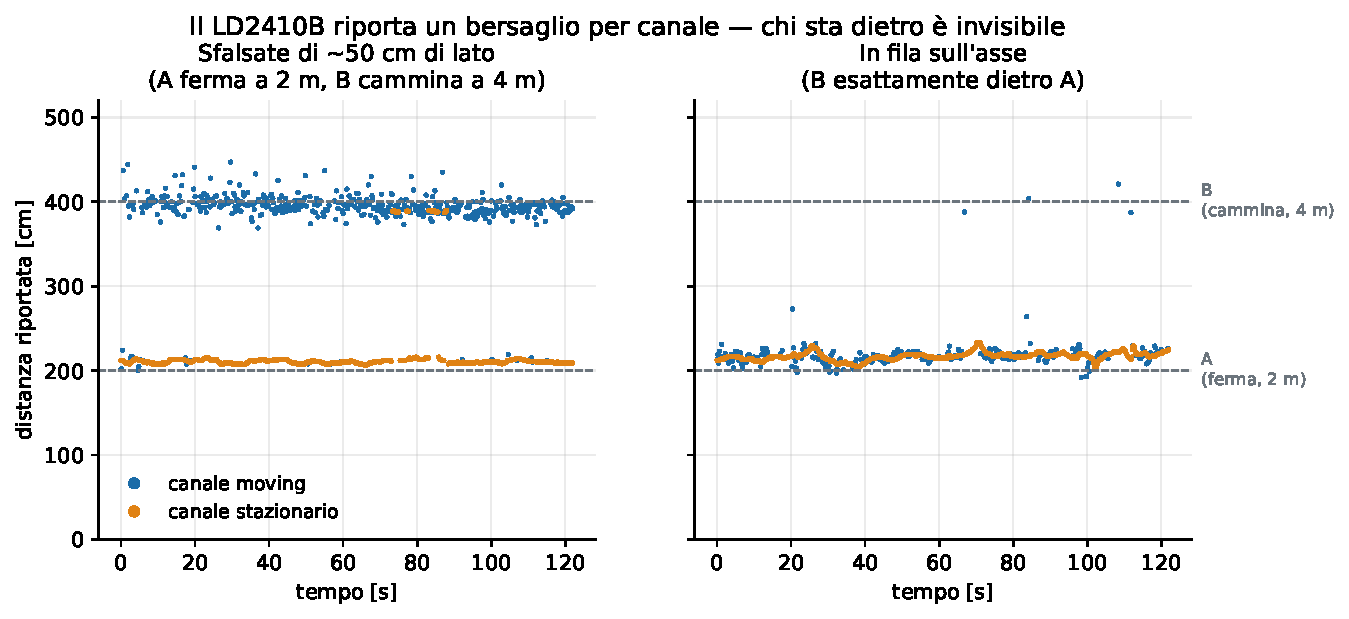
\includegraphics[width=\linewidth]{figures/fig08_due_persone}
\caption{Due persone davanti al radar in tre geometrie. Il modulo riporta un
bersaglio per canale, quindi separa bene due persone in stati diversi, male due
persone ferme, per nulla una persona dietro l'altra. La presenza resta al 100\,\% in
ogni caso.}
\label{fig:due-persone}

\end{figure}

Il limite del modulo va quindi formulato dicendo che riporta un bersaglio per canale.
Con A ferma
e B in movimento i due canali sono attivi insieme nel 79\,\% dei campioni e riportano
due distanze separate da 177~cm. L'energia in movimento (38,4) è coerente con quella
misurata a 4~m nella caratterizzazione della distanza (35,1). Con entrambe ferme i
due bersagli competono per lo stesso canale e la più vicina vince nel 93\,\% dei
campioni, anche se B compare comunque nel 19,5\,\% grazie ai suoi micro-movimenti
involontari.
In fila il corpo davanti nasconde del tutto quello dietro, e i due canali riportano lo
stesso bersaglio, con differenza mediana di 3~cm. In ogni geometria la presenza è al
100\,\%, quindi il radar non sbaglia mai a dire che c'è qualcuno e ciò che perde è il
conteggio. Per il progetto questo rafforza l'architettura a un sensore per arredo, dove
ogni sensore ha un solo bersaglio, ed esclude invece l'uso di un sensore singolo come
contatore di presenze in aula.

\paragraph{Il secondo radar.} L'\ldc\ ha un solo canale di bersaglio
(Sezione~\ref{sec:c3-2}), e la prova ripetuta con A ferma a 1~m e B a 2~m lo mostra. La
presenza è al 100\,\% in tutte le geometrie, ma non esiste un canale su cui B possa
comparire. In fila B è invisibile come sull'\ldb, mentre con le persone sfalsate le
energie per gate non le separano. La distanza riportata si aggancia a B quando B è in
movimento (211--214~cm in due trial su tre) e resta piantata su un valore fisso
(268~cm) con entrambe ferme. Il secondo radar dice che c'è qualcuno e non quanti,
anche nella geometria in cui l'\ldb\ riporta la seconda persona nel 74\,\% dei
campioni.

\section{Penetrazione degli ostacoli}
\label{sec:ostacoli}

Il pannello è interposto a 20~cm dal sensore, perpendicolare all'asse e libero di
reggersi da solo. Serve un soggetto in movimento sul posto, perché su un bersaglio
fermo il canale stazionario satura e l'attenuazione non sarebbe osservabile. Servono
anche due distanze, 3~m per l'\ldb, dove l'energia vale circa metà scala, e 1~m per
il PIR, che a 3~m non rileva il movimento sul posto. L'\ldc\ ha ripetuto la serie a
1~m, l'unica distanza a cui l'esemplare lavora. Le sue energie sono interi a 16~bit
che lo strumento del produttore mostra in decibel, quindi la sua attenuazione è
espressa come $10\log_{10}(E_0/E)$ sul gate della persona. È un'ipotesi dichiarata,
perché il produttore non documenta il campo. Il riferimento senza ostacolo è la media
di sei trial a inizio e fine sessione, perché la baseline è la misura meno
riproducibile della serie (da 47,8 a 57,3 sull'\ldb). I risultati sono in
Tabella~\ref{tab:ostacoli} e Figura~\ref{fig:attenuazione}.

\subsection{Attenuazione per materiale}
\label{sec:ostacoli-materiali}
\label{sec:ld2420-attenuazione}

\begin{table}[htbp]
\centering
\caption{Attenuazione per materiale sui due radar e rilevamento del PIR a 1~m. \ldb:
riduzione dell'energia del bersaglio in movimento a 3~m rispetto alla baseline
mediata (53,45), in unità dello strumento. \ldc: attenuazione in decibel del gate~2
grezzo a 1~m (fondo 13). Legno e metallo sono al fondo, perché la dinamica dell'esemplare è di 5~dB. I pannelli hanno inoltre coperture angolari diverse ($\pm 42$ a $\pm 70$\textdegree), quindi tutte le attenuazioni sono limiti inferiori. Il confronto più pulito è legno contro cartone, entrambi a
$\pm 54$\textdegree.}
\label{tab:ostacoli}

\small
\begin{tabular}{@{}llrrr@{}}
\toprule
\textbf{Materiale} & \textbf{Spessore} & \textbf{\ldb\ (3~m)} & \textbf{\ldc\ (1~m)} & \textbf{PIR (1~m)} \\
\midrule
Nessuno (riferimento) & --- & --- & --- & $79{,}6\,\%$ \\
Plastica (tanica cava) & $2 \times 5$~mm + aria & $-7{,}5\,\%$ & 0,4~dB & $0\,\%$ \\
Cartongesso & 10~mm & $-26\,\%$ & \textbf{0,7~dB} & $0\,\%$ \\
Cartone (scatola) & $2 \times 5$~mm + aria & $-17{,}2\,\%$ & 1,0~dB & $0\,\%$ \\
Vetroresina & 1~mm & $-19{,}6\,\%$ & 1,0~dB & $0\,\%$ \\
Vetro & 5~mm & $-40{,}9\,\%$ & 2,4~dB & $\sim 0\,\%$ \\
Legno & 10~mm & $-41{,}6\,\%$ & $\geq 4{,}1$~dB & $\sim 0\,\%$ \\
Metallo & 1~mm & \textbf{blocca} & $\geq 5{,}5$~dB & $0\,\%$ \\
\bottomrule
\end{tabular}
\end{table}

\begin{figure}[htbp]
\centering
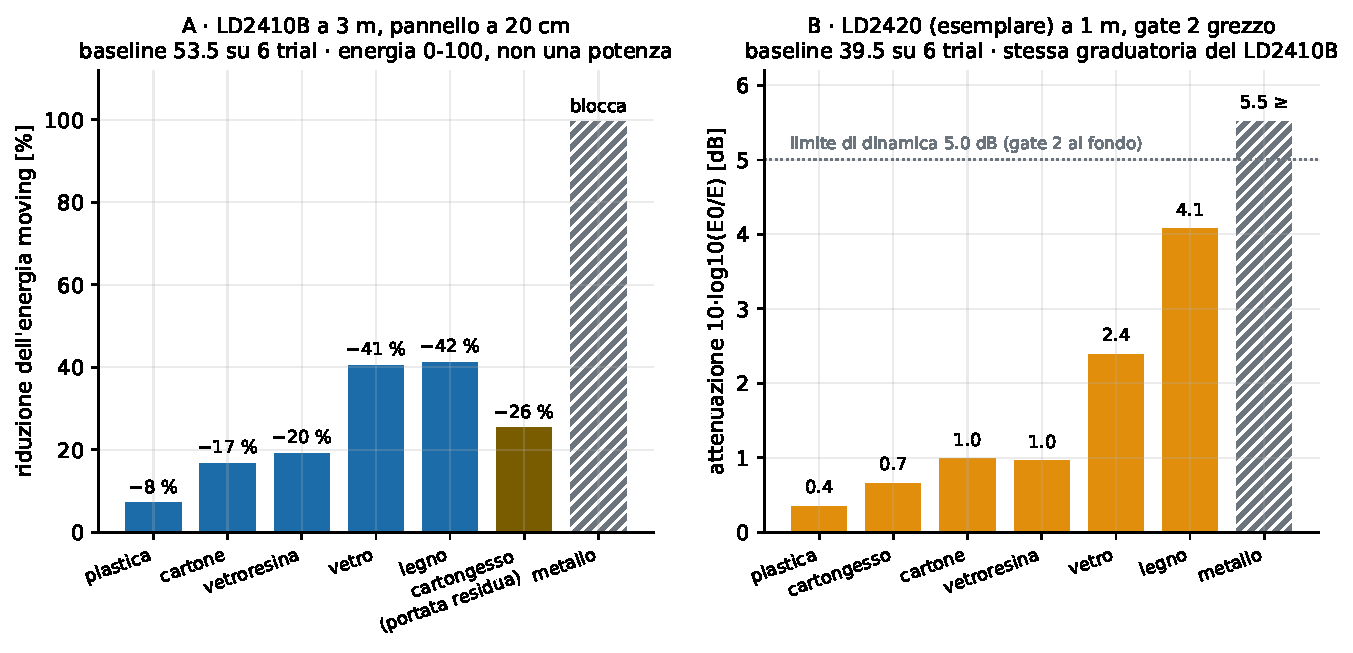
\includegraphics[width=\linewidth]{figures/fig15_attenuazione_materiali}
\caption{Attenuazione per materiale sui due radar, pannello a 20~cm dal sensore. A:
\ldb\ a 3~m, riduzione dell'energia in movimento. Vale la graduatoria dei materiali, non il valore. B: \ldc\ a 1~m, energie grezze a 16~bit in decibel. Legno e metallo sono limiti inferiori.}
\label{fig:attenuazione}

\end{figure}

L'\ldb\ rileva la presenza nel 100\,\% dei campioni attraverso tutti i materiali
dielettrici, con attenuazioni fra il 7 e il 42\,\% dell'energia, mentre il PIR è
azzerato da ognuno di essi. Il caso più immediato è quello del vetro, un materiale
trasparente alla luce visibile che il radar attraversa e che per il PIR è opaco, perché il vetro comune
non trasmette oltre i 4--5~\textmu m mentre l'emissione del corpo è centrata sui 10.
La graduatoria è identica sui due radar, a due distanze e in due unità (plastica,
cartone e vetroresina, vetro, legno, metallo). Il cartongesso, il materiale delle
pareti di un'aula, attenua come plastica e cartone. Con il metallo l'\ldb\ riporta un
bersaglio a 30,0~cm con dispersione nulla, cioè il pannello stesso, e del soggetto non
resta traccia, il che prova anche che l'aggiramento del pannello è sotto soglia. Sull'\ldc\ la frazione di campioni sopra la
soglia di mantenimento del gate~2 passa dal 25--33\,\% senza ostacolo allo 0--1\,\%
dietro 10~mm di legno. Quell'esemplare non acquisirebbe quindi una persona a 1~m
dietro un pannello di legno, dove l'\ldb\ a 3~m è al 100\,\%.

\subsection{Portata residua con l'ostacolo}
\label{sec:ostacoli-portata}

Le percentuali non rispondono alla domanda
pratica del relatore, cioè fin dove arriva con una porta di mezzo un radar che senza
ostacolo arriva a 5~m. L'\ldb\ ha quindi ripetuto la geometria percorrendo le distanze da 1
a 5~m con il cartongesso, e a 3--5~m con legno, vetro e una porta interna chiusa
(tamburata, senza vetro, con il sensore all'interno a 20--30~cm dal battente), tre
trial per punto (Figura~\ref{fig:portata-ostacoli}). Nessun dielettrico accorcia la portata
entro i 5~m della stanza, e in tutti i 39 trial con ostacolo, porta compresa, la
presenza è al 100\,\% e la distanza è corretta. Ciò che degrada è il canale in
movimento, la cui frazione di campioni attivi a 5~m passa dal 78\,\% senza ostacolo al
44 con il cartongesso, 26 con il vetro, 19 con il legno e 3\,\% con la porta, mentre la
presenza la tiene il canale stazionario. La porta è trasparente a 3~m (energia pari
alla baseline) e quasi opaca a 5, più del legno pieno, e il fenomeno non è spiegato.
Nella stessa sessione il PIR a 1~m passa dal 44--97\,\% senza ostacolo allo 0\,\% con il cartongesso.

\begin{figure}[htbp]
\centering
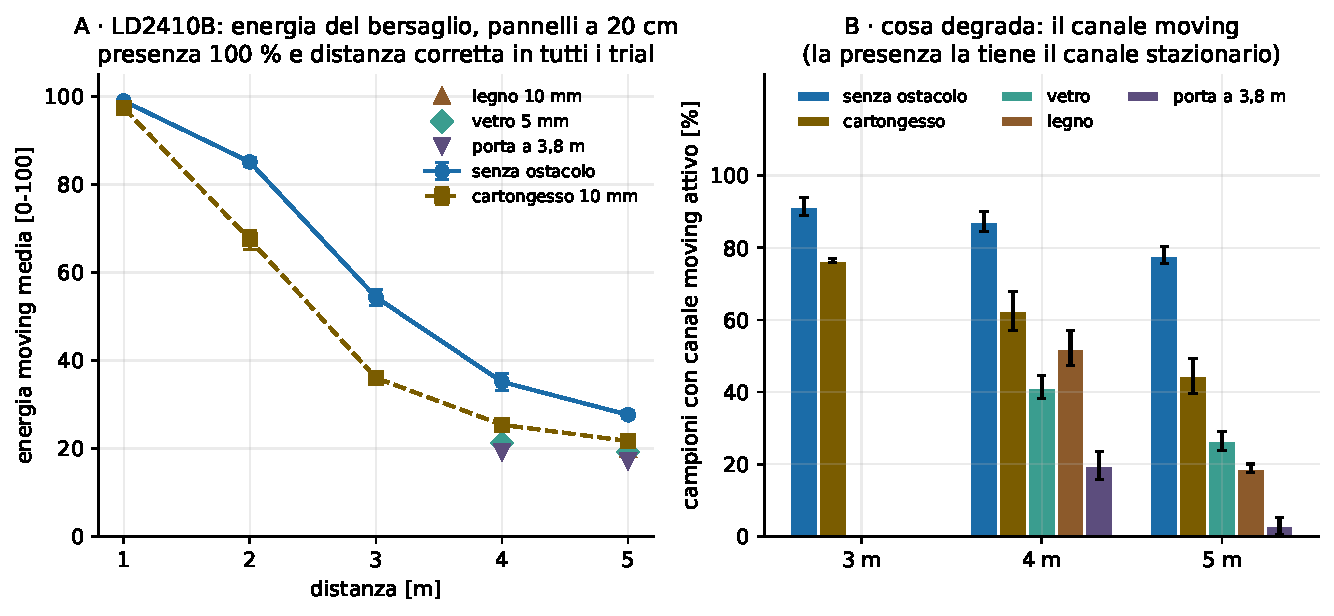
\includegraphics[width=\linewidth]{figures/fig14_portata_ostacoli}
\vspace{2.3cm}% spazio per la didascalia nel margine (tufte non lo riserva)
\caption{\ldb, portata residua con l'ostacolo a 20~cm dal sensore. A: energia in
movimento con cartongesso a 1--5~m e con legno, vetro e porta chiusa a 3--5~m. B: frazione di campioni con il canale in movimento attivo.}
\label{fig:portata-ostacoli}

\end{figure}

Per il progetto questo significa che il sensore può essere incassato nell'arredo,
dietro legno o cartongesso o dentro un guscio di vetroresina, mentre il PIR deve affacciarsi direttamente sull'ambiente. Il metallo resta l'unico vincolo assoluto, e nel banco
reale la lamiera di rinforzo sta dietro al modulo e non davanti.

\section{Portata massima in corridoio}
\label{sec:portata-massima}

A 5~m nessuno dei tre sensori aveva mostrato il proprio limite in stanza. La prova di
portata è stata quindi svolta per ultima in un corridoio largo 120~cm
(Figura~\ref{fig:geometrie}d), con i sensori a 80~cm da terra e i punti a 6, 7 e 8~m visti
attraverso due vani porta. Venti minuti di corridoio vuoto non producono alcun evento
su radar e PIR. Il fondo dei gate lontani dell'\ldb\ ha massimo 7 contro una soglia di
15, quindi vani e muro di fondo non compaiono. I risultati dei tre sensori sono
riassunti in Figura~\ref{fig:portata-tre-sensori}.

\begin{figure}[htbp]
\centering
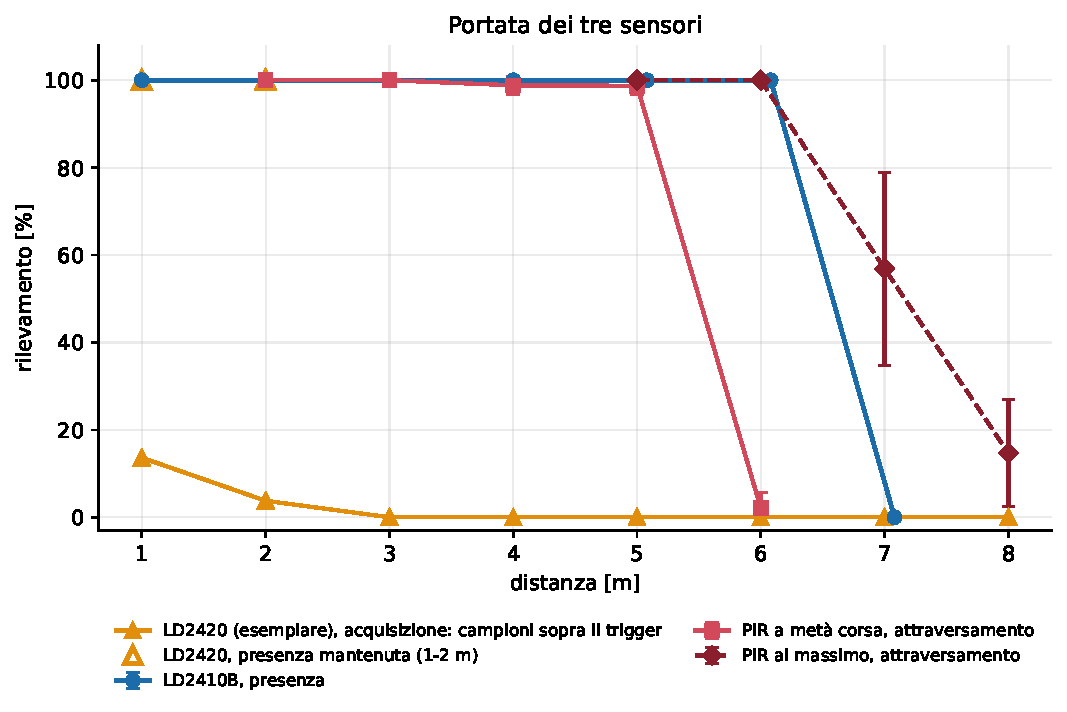
\includegraphics[width=\linewidth]{figures/fig17_portata_tre_sensori}
\caption{Portata dei tre sensori sulla stessa scala, in stanza fino a 5~m e in corridoio fino a 8~m. \ldb: 100\,\% fino a 6~m, zero a 7 per il tetto configurato. PIR a metà
corsa: attraversamento a circa 1~m/s rilevato fino a 5~m, quasi nullo a 6. Al massimo
di sensibilità 100\,\% a 5--6~m, 57\,\% a 7, 15\,\% a 8. \ldc\ (esemplare): si accende
entro 1~m (triangoli pieni) e mantiene la presenza fino a 2~m (triangoli vuoti).}
\label{fig:portata-tre-sensori}

\end{figure}

\paragraph{\ldb.} Con un'oscillazione trasversale sul posto di circa 50~cm il radar
rileva al 100\,\% a 5 e 6~m e allo 0\,\% a 7~m in tre trial su tre. A 6~m la distanza
riportata ha massimo esattamente 600~cm in cinque trial su cinque, con dispersione di
2--5~cm contro i 10--11 di 5~m. Non si tratta di una misura più precisa, ma del tetto
degli otto gate da 75~cm configurati. La presenza a 6~m è retta dal canale stazionario
(energia 62--82), mentre a 7~m i gate 7 e 8 restano molto sotto le soglie. Il tetto di
600~cm dichiarato dal manuale risulta così misurato, e il punto a 6~m non entra nella
regressione della distanza perché saturo.

\paragraph{PIR.} A metà corsa, la sensibilità di tutta la campagna, l'oscillazione
trasversale è rilevata al 24--33\,\% anche a 7~m, dove il radar per configurazione non
vede nulla. L'attraversamento vero a circa 1~m/s dà 0, 6 e 0\,\% a 6~m contro il
98,7\,\% di 5~m. Un transito più veloce alla stessa distanza dà il 30\,\% con cinque
impulsi. Al limite della portata la velocità del transito decide, al pari del tipo e
dell'ampiezza del movimento. Con il trimmer al massimo l'attraversamento è rilevato al
100, 100, $56{,}8 \pm 18{,}0$ e $14{,}7 \pm 10{,}0\,\%$ a 5, 6, 7 e 8~m. Il limite sta
fra 7 e 8~m, coerente con i 3--7~m del datasheet. Oltre il tetto del radar il PIR al
massimo vede ancora, ma solo chi attraversa il suo campo abbastanza in fretta. La
serie al massimo è dichiaratamente separata dal resto della campagna.

\paragraph{\ldc.} Con il gate massimo portato a 12 (840~cm), il valore di fabbrica
che copre gli 8~m dichiarati, l'esemplare acquisisce a 1~m e mantiene a 2~m. Da 3~m in
su le sue energie sono il fondo del corridoio vuoto gate per gate. Il gate massimo non
ha quindi aggiunto nulla, e il limite è dell'esemplare e non della configurazione né
della stanza.

Per un sensore sotto un banco i 6~m dell'\ldb\ sono molto più del necessario, e la domanda di
progetto va nella direzione opposta, cioè come restringere il campo (Sezione~\ref{sec:angolare}).

\section{Il secondo radar: che cosa cambia}
\label{sec:ld2420-risultati}
\label{sec:ld2420-taratura}
\label{sec:ld2420-fp}
\label{sec:ld2420-dipme}
\label{sec:ld2420-limiti}
\label{sec:ld2420-latenze}
\label{sec:ld2420-angolare}

La campagna sul secondo radar segue il protocollo della Sezione~\ref{sec:protocollo-ld2420}. I
suoi risultati test per test sono già nelle figure delle sezioni precedenti. Questa
sezione raccoglie ciò che cambia rispetto all'\ldb, e la Tabella~\ref{tab:ld2420-sintesi}
li riassume.

\paragraph{La taratura è una condizione necessaria.} La Sezione~\ref{sec:c3-6} spiega perché a
configurazione di fabbrica il modulo non rilascia mai la presenza nella stanza di
prova. Le misure lo quantificano. Il muro a circa 5~m sta nel gate~7 e supera la
soglia di mantenimento nel 4\,\% dei campioni, e con un ritardo di scomparsa di 30~s
basta un superamento ogni mezzo minuto. La soglia di mantenimento del gate~5 esce
dalla scansione dello strumento a 13,8~dB in tre scansioni, contro un fondo misurato
su 120~s con media 15 e massimo 34.

\paragraph{Falsi positivi.} Le 181 riaccensioni in 7~h di Sezione~\ref{sec:falsi-positivi}
hanno una firma precisa, episodi di 31,8~s mediani, cioè un trigger isolato più i 30~s
di ritardo. L'attribuzione per gate indica il gate~0 in 80 casi su 181, e il gate~0 è
l'accoppiamento fra trasmettitore e ricevitore, non una distanza. Portando il solo
gate~0 sopra la coda del rumore, un'ora di giorno dà 5 riaccensioni, cioè 5,4 eventi/h. Il
residuo viene dai gate 1 e 2, che non si possono alzare perché sono quelli in cui la
persona a 50~cm e a 1~m produce il suo segnale con margine quasi nullo. Su questo
esemplare rumore e persona si sovrappongono, e 5,4 eventi/h è un pavimento
strutturale. Il modulo inoltre stima il fondo all'accensione, quindi un corpo a 20~cm
nei primi 60~s lo lascia in presenza permanente senza risposta alla persona, finché non
viene spento per un quarto d'ora. L'\ldb\ non l'ha mai fatto in decine di riavvii.

\paragraph{Nessuna grandezza continua.} La dose-risposta di Sezione~\ref{sec:dose-risposta},
ripetuta sull'\ldc\ nella stessa geometria, non gradua il movimento. L'energia del
gate~2 vale 13,4 a stanza vuota, $41{,}0 \pm 9{,}3$ da immobile, $34{,}8 \pm 1{,}0$
con i micro-movimenti e 31,0 in cammino. L'ordine è rovesciato rispetto all'\ldb\ e le condizioni si sovrappongono. Il canale separa vuoto da
occupato e poi non distingue. Su questo esemplare non esiste quindi la grandezza da
cui costruire l'indice di vitalità.

\paragraph{Gate minimo.} Il gate minimo è l'unica funzione che l'\ldc\ ha e
l'\ldb\ no, ma non tocca la decisione di presenza (100\,\% con la persona nel gate
escluso) e confina la distanza al bordo della finestra.

\paragraph{Respiro.} Con il metronomo a 15 atti al minuto a 1~m, il criterio della
Sezione~\ref{sec:respiro} recupera la frequenza in un trial su tre (due su tre a gate
fissato), con controlli negativi puliti, contro 13 su 15 dell'\ldb. La persona occupa
due gate soli contro i 7--14 canali concordi dell'\ldb, e il rapporto segnale-rumore
massimo è 6,1 contro 12,8. La saturazione è zero, ma il vantaggio dei 16~bit è
annullato dal segnale debole dell'esemplare.

\begin{table}[htbp]
\centering
\caption{I due radar a confronto, tutte grandezze misurate in questa tesi. Le righe
dell'\ldc\ si riferiscono all'esemplare in dotazione, con soglie tarate.}
\label{tab:ld2420-sintesi}

\small
\begin{tabularx}{\linewidth}{@{}Xll@{}}
\toprule
\textbf{Grandezza} & \textbf{\ldb} & \textbf{\ldc\ (esemplare)} \\
\midrule
Funziona a soglie di fabbrica nella stanza di prova & sì & no, presenza permanente \\
Falsi positivi a stanza vuota & $\leq 0{,}43$/h (0 in 6,6~h) & 26,2/h tarato, 5,4/h con gate~0 alzato \\
Portata su persona in movimento & 6~m (tetto configurato) & 1~m acquisizione, 2~m mantenimento \\
Persona immobile a 1~m / sotto il banco & $100\,\%$ / $100\,\%$ & $100\,\%$ / $98{,}4\,\%$ \\
Distanza su bersaglio fermo & sì, dispersione 1,5~cm & no (manuale \S8, misurato) \\
Distanza su bersaglio in moto & continua fino a 5~m, $R^2 = 0{,}99965$ & valida fino a 1~m, poi stantia \\
Graduazione del movimento & 68,6, 84,4, 99,3 & piatta e rovesciata \\
Latenza d'ingresso & $5{,}36 \pm 0{,}30$~s & $7{,}28 \pm 1{,}40$~s \\
Rilascio (parametro 5~s) & $18{,}4$~s & $7{,}7$~s (campo più corto) \\
Copertura angolare a 1~m & $\geq \pm 90$\textdegree & $\approx \pm 75$\textdegree \\
Cartongesso 10~mm & $-26\,\%$ a 3~m, portata intatta & 0,7~dB \\
Legno 10~mm & $-42\,\%$, portata intatta & non acquisirebbe a 1~m \\
Respiro a ritmo imposto & 13/15 trial & 1/3 (2/3 a gate fisso) \\
Due persone & un bersaglio per canale & un bit \\
Comportamento all'avvio & stabile in decine di riavvii & fondo corrotto da un corpo vicino \\
\bottomrule
\end{tabularx}
\end{table}

\paragraph{Un riscontro indipendente.}
\label{sec:ld2420-riscontro}
Una relazione di progetto svolta a Camerino nello stesso anno accademico arriva a
conclusioni sovrapponibili, con un altro esemplare di ciascun modulo, un'altra libreria
e un altro protocollo sperimentale~\cite{dellaquila2026}. Sull'\ldc\ riporta un flag di
presenza inaffidabile, un primo gate con energie alte anche a stanza vuota ed escluso
dalla logica, la necessità di tarare le soglie per gate e, anche dopo, la
sovrapposizione fra stanza vuota e soggetto poco attivo. Sull'\ldb\ non osserva falsi
positivi con finestre aperte, tende mosse dal vento e in ambiente esterno, e giudica
stabile la presenza per tutta la permanenza del soggetto. Le differenze sono due. La
relazione giudica buona l'accuratezza di distanza dell'\ldc, coerente con
l'attribuzione all'esemplare del nostro limite di portata. Giudica inoltre l'\ldb\
inadatto al respiro, ma legge la distanza con il modulo sul torace, mentre qui si
legge l'energia per gate a 2~m.

\paragraph{La lettura per il progetto.} Nello scenario DIPME l'\ldc\ rileva la
persona immobile sotto il banco, e questo va detto. Ma dice se e non dove, non gradua
il movimento, richiede una taratura per installazione, che su centinaia di banchi è un costo operativo sostanziale, e conserva 5,4 riaccensioni l'ora. L'\ldb\ funziona a soglie di fabbrica con zero falsi positivi, riporta la
distanza anche sul bersaglio fermo e fornisce la grandezza continua da cui nasce
l'indice di vitalità. Un secondo esemplare di \ldc\ permetterebbe di separare i limiti
del modello da quelli del pezzo.

\section{Sintesi del confronto}
\label{sec:discussione}

La Tabella~\ref{tab:sintesi} raccoglie in una sola vista i risultati del capitolo. Tutte le
righe con soggetto in movimento o con micro-movimenti sono acquisite con il PIR nella
configurazione a lui più favorevole.

\begin{table}[htbp]
\centering
\caption{Sintesi della campagna sperimentale. ``Rilev.'' è la frazione di campioni in
cui il sensore riporta la presenza, con la ground truth indicata. La colonna del radar si riferisce all'\ldb, mentre l'\ldc\ è riassunto nella Tabella~\ref{tab:ld2420-sintesi}.}
\label{tab:sintesi}

\small
\begin{tabularx}{\linewidth}{@{}llrrX@{}}
\toprule
\textbf{Scenario} & \textbf{Verità} & \textbf{Rilev.\ PIR} & \textbf{Rilev.\ radar} &
\textbf{Riferimento} \\
\midrule
Stanza vuota, 7,03~h & assente & $0$ ev/h & $0$ ev/h & Sezione~\ref{sec:falsi-positivi} \\
Fermo seduto, 2,3~m & presente & $0{,}22\,\%$ & $\mathbf{100\,\%}$ & Sezione~\ref{sec:persona-ferma} \\
Fermo in piedi, 1~m & presente & $1{,}52\,\%$ & $\mathbf{100\,\%}$ & Sezione~\ref{sec:dose-risposta} \\
Micro-movimenti, 1~m & presente & $51{,}60\,\%$ & $\mathbf{100\,\%}$ & Sezione~\ref{sec:dose-risposta} \\
Cammino sul posto, 1~m & presente & $85{,}20\,\%$ & $\mathbf{100\,\%}$ & Sezione~\ref{sec:dose-risposta} \\
Cammino sul posto, 2--5~m & presente & $0{,}00\,\%$ & $\mathbf{100\,\%}$ & Sezione~\ref{sec:dose-risposta} \\
Attraversamento 1--5~m & presente & $99$--$100\,\%$ & $\mathbf{100\,\%}$ & Sezione~\ref{sec:dose-risposta} \\
Sotto il banco, immobile & presente & $1{,}32\,\%$ & $\mathbf{100\,\%}$ & Sezione~\ref{sec:sotto-banco} \\
Sotto il banco, micro-mov. & presente & $96{,}52\,\%$ & $\mathbf{100\,\%}$ & Sezione~\ref{sec:sotto-banco} \\
Due persone, ogni geometria & presenti & --- & $\mathbf{100\,\%}$ & Sezione~\ref{sec:due-persone} \\
Vicino a 3~m, gate 2 & assente & $0{,}00\,\%$ & $0{,}00\,\%$ & Sezione~\ref{sec:angolare} \\
Vicino fermo a 90\textdegree, gate 2 & assente & $0{,}00\,\%$ & $0{,}00\,\%$ & Sezione~\ref{sec:angolare} \\
Vicino a 90\textdegree\ in movimento & assente & $12\,\%$ & $\mathbf{100\,\%}$ & Sezione~\ref{sec:angolare} \\
Dietro cartongesso, legno, vetro, porta, 3--5~m & presente & $0\,\%$ (1~m) & $\mathbf{100\,\%}$ & Sezione~\ref{sec:ostacoli} \\
Corridoio 6~m / 7~m, oscillazione & presente & $12$--$51$ / $24$--$33\,\%$ & $\mathbf{100\,\%}$ / $0\,\%$ & Sezione~\ref{sec:portata-massima} \\
Attraversamento 6~m, PIR al massimo & presente & $\mathbf{100\,\%}$ & $100\,\%$ & Sezione~\ref{sec:portata-massima} \\
\bottomrule
\end{tabularx}
\end{table}

\subsection{Dove il mmWave vince}
\label{sec:mmwave-vince}
\begin{itemize}[leftmargin=1.4em,itemsep=2pt]
  \item Sulla persona ferma il divario è categorico, non graduale. A 2,3~m seduto,
        a 1~m in piedi e sotto il banco a 60~cm il PIR ha il 98,5--99,8\,\% di falsi
        negativi e il radar lo 0,00\,\%, cioè lo stesso esito in tre geometrie.
  \item Il divario è attribuibile a una sola variabile, l'immobilità del soggetto,
        perché la dose-risposta la isola a geometria, distanza e configurazione
        costanti.
  \item Il radar è più veloce anche dove il PIR dovrebbe essere avvantaggiato,
        all'ingresso da una porta, in dieci trial su dieci.
  \item Il radar aggiunge informazione, non solo affidabilità. La distanza è lineare
        con $R^2 = 0{,}99965$, mentre l'energia e la dispersione della distanza sono
        indicatori continui della quantità di movimento.
  \item Sui falsi positivi i due sensori sono equivalenti ($\leq 0{,}43$ eventi/h).
        Il radar attraversa cartongesso, legno, vetro e una porta chiusa senza perdere
        portata, mentre il PIR è azzerato da ogni materiale.
\end{itemize}

\subsection{Dove il mmWave non vince}
\label{sec:mmwave-non-vince}
\begin{itemize}[leftmargin=1.4em,itemsep=2pt]
  \item Il consumo, tre ordini di grandezza in più (80~mA contro 50~\textmu A), è il
        vincolo che determina l'architettura del Capitolo~\ref{chap:conclusioni} e che il
        Capitolo~\ref{chap:consumi} quantifica.
  \item Il rilascio è più lento del PIR di 5,4~s e più lento del parametro
        dichiarato (coda di circa 9~s contro 5~s configurati).
  \item A distanza ravvicinata i canali più informativi saturano e i gate stazionari
        non sono disponibili sotto 1,5~m. Sotto l'arredo la localizzazione è dieci
        volte più rumorosa, anche se la presenza resta al 100\,\%.
  \item Riporta un bersaglio per canale, quindi non è un contatore di presenze.
        Richiede UART, protocollo a frame ed elaborazione numerica contro il piedino
        digitale del PIR.
  \item I vantaggi misurati sono dell'\ldb\ e non della categoria mmWave in astratto, come mostra il secondo radar (Sezione~\ref{sec:ld2420-risultati}).
\end{itemize}

\subsection{Limiti del setup}
\label{sec:limiti}

Tutti i risultati comparativi sono di un solo soggetto,
in una stanza domestica e non in un'aula, a una temperatura sfavorevole al PIR
(Sezione~\ref{sec:registro}). C'è un solo esemplare per modello e nessuna strumentazione di
misura indipendente per distanze e consumi. Gli scenari di selettività e a due persone
hanno tre trial soli (Tabella~\ref{tab:scenari}), e su tre trial le affermazioni sono
formulate come assenza di effetto osservato. La prima parte della campagna è in posizione L del PIR (Sezione~\ref{sec:interpretazione-pir}), e i due gruppi non sono uniti nella regressione della distanza perché separati da un rimontaggio del setup. Nessuno di questi limiti tocca il risultato centrale, perché la cecità del PIR sulla persona ferma è una conseguenza del principio fisico, confermata in tre geometrie.
